\documentclass[10pt,twocolumn, nofootinbib]{revtex4-2}
%\documentclass[aps,pra,10pt,twocolumn,floatfix,nofootinbib]{revtex4-1}
%\documentclass[10pt,twocolumn,letterpaper]{article}

\usepackage{assumptionsofphysics}
\usepackage{graphicx}
\usepackage{hyperref}
\hypersetup{
	colorlinks=true,
	citecolor=blue,
	urlcolor=blue,
	linkcolor=blue
}
\urlstyle{same}
\frenchspacing

\newcommand\partitle[1]{\textsc{#1}.}


\begin{document}

\title{Geometrical and physical interpretation of the action principle}
\author{Gabriele Carcassi, Christine A. Aidala}
\affiliation{Physics Department, University of Michigan, Ann Arbor, MI 48109}

\date{\today}


\begin{abstract}
We give a geometrical interpretation for the action principle in Lagrangian classical particle mechanics that also has a direct physical meaning. The idea is that the variation of the action along a path is the flow of the displacement field through the area between the path and the variation. Since actual trajectories are parallel to the displacement field, the flow is zero along them, making the action stationary. We first give the interpretation for a single degree of freedom using simple differential calculus so that it is accessible to the widest possible audience. We then generalize to multiple degrees of freedom using symplectic geometry. This treatment makes the geometry of both Hamiltonian and Lagrangian mechanics more readily evident, and gives reasons to privilege the Hamiltonian picture over the Lagrangian one.
\end{abstract}

\maketitle

\section{Introduction}

While the principle of stationary action is regarded by many as one of the most important tools in physics, its physical meaning is not completely clear. First of all, the typical characterization of the Lagrangian as the difference between kinetic and potential energy fails even for simple systems, like a charged particle under a magnetic field. Moreover, the Lagrangian for a system is not uniquely defined, making the actual value of the action for a path not directly physically significant.  We are left to wonder: what exactly is the action and why is it stationary for actual trajectories?

As part of our larger project Assumptions of Physics, we developed an approach, called Reverse Physics, which examines current theories to find a set of starting physical assumptions that are sufficient to rederive them. This allowed us to recast Hamiltonian mechanics as the dynamics of deterministic and reversible evolution, which coincidentally gives us the proper setting to characterize both the physics and the geometry underlying the principle of stationary action. We will see that the principle arises as a feature of divergence-free fields and closed two-forms, as a general mathematical property of vector calculus and differential geometry.

We will first address the case of a single degree of freedom using standard vector calculus. This provides already all the geometrical and physical insights in a language that is accessible to all physicists and engineers. Then we proceed to the case of multiple independent degrees of freedom, which requires tools from differential geometry. To make the treatment of the latter case more accessible, we will use a notation that is similar to the one used by physicists in general relativity.

\section{One degree of freedom}

The first thing we need to do is recast the equations of motion in a form that will make apparent both their geometrical interpretation and their physical meaning. The setting is phase space extended with the time variable. That is, the space charted by position $q$, momentum $p$ and time $t$. It is precisely because we have exactly three variables that the standard tools of vector calculus can be used.

\begin{figure}
	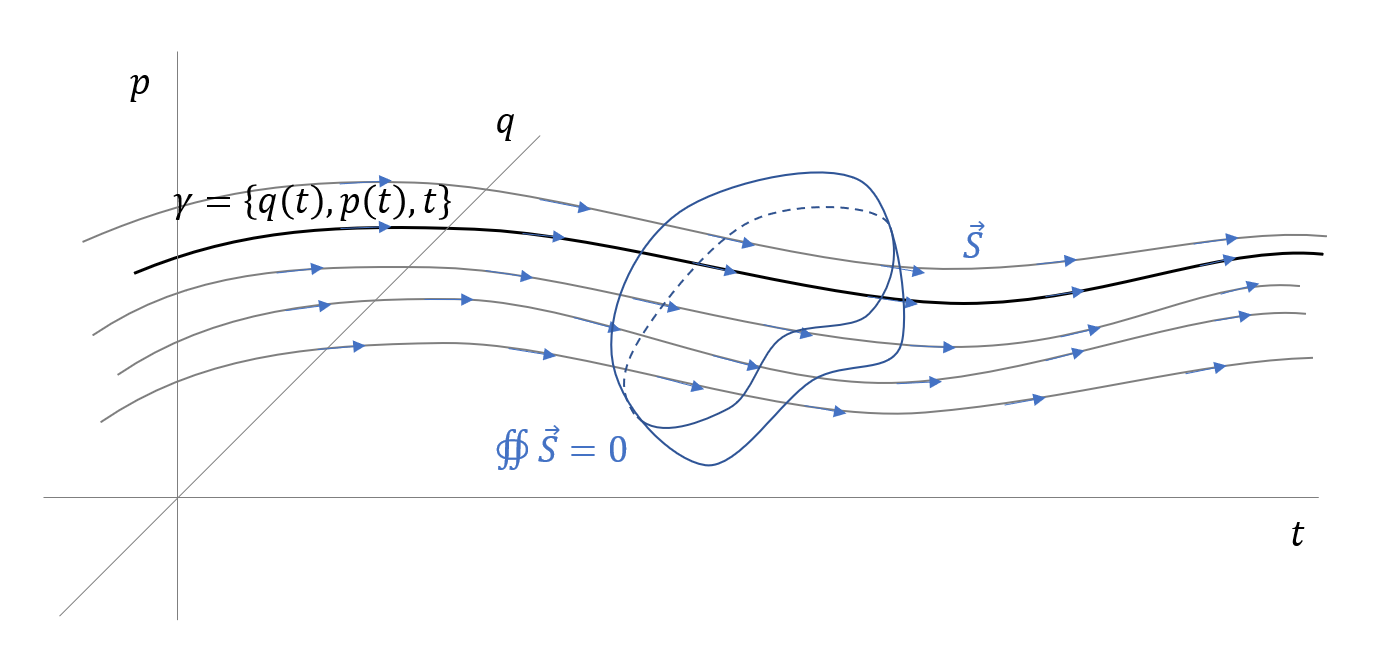
\includegraphics[width = 0.45\textwidth]{ExtendedPhaseSpace}
	\caption{\footnotesize{Evolutions in the extended phase space and the divergence-free displacement field.}}\label{extended_phase_space}
\end{figure}


Once we have recast the equations of motion on the extended phase space, we can see how the action principle comes from a straightforward application of vector calculus in the case of divergence-free fields.

\subsection{Hamiltonian reformulation}

Let us quickly review the equations for a Hamiltonian system with a single degree of freedom in the extended phase space. We can chart all states at all times by using three variables, $\{q,p,t\}$. Given a set of initial conditions $\{q_0,p_0,t_0\}$, we can find a single evolution $\gamma = \{q(t), p(t), t\}$ by solving Hamilton's equations:
\begin{equation}\label{Hamilton_equations}
\begin{aligned}
	\frac{dq}{dt} &= \frac{\partial H}{\partial p} \\
	\frac{dp}{dt} &= -\frac{\partial H}{\partial q}.
\end{aligned}
\end{equation}
How can we better understand the physics and geometry captured by these equations?

Let us step back, and forget we have a Hamiltonian system. Suppose we simply have a system described by a single degree of freedom and assume the following:
\begin{align}\label{Detrev_assumptions}
	\parbox{2.8in}{the system undergoes deterministic and reversible evolution.}
\end{align}

Under this assumption, given a state at a moment in time, there is a well-defined change in all variables which is described by the displacement vector field
\begin{equation}
	\vec{S} = \left\{ \frac{dq}{dt},\frac{dp}{dt},\frac{dt}{dt} \right\}.
\end{equation}
If we consider a finite region in the extended phase space, given that the evolution is deterministic and reversible we expect the number of states flowing in and flowing out of the region to be the same. Equivalently, we expect the evolutions to neither converge or diverge. Mathematically, the displacement field must be divergence-free, that is
\begin{equation}
	\nabla \cdot \vec{S} = 0,
\end{equation}
to properly represent a deterministic and reversible evolution.

Since $\vec{S}$ is divergence-free, we can find a vector potential
\begin{equation}
	\vec{\theta} = \{\theta_q, \theta_p, \theta_t\}
\end{equation}
such that
\begin{equation}\label{displacement_has_potential}
	\vec{S} = - \nabla \times \vec{\theta}.
\end{equation}
The minus sign is introduced to match conventions in differential geometry. Mathematically, this is analogous to what is done for a magnetic field or for an incompressible fluid.

Given that $\vec{\theta}$ is a vector potential, we have the usual gauge arbitrariness since $\nabla \times(\vec{\theta} + \nabla f) = \nabla \times \vec{\theta}$ and therefore the displacement field $\vec{S}$ remains unchanged. By choosing $f(q,p,t)$ appropriately, we can set
\begin{equation}
	\vec{\theta} = \{\theta_q, 0, \theta_t\}
\end{equation}
without loss of generality.

The displacement field has a further constraint, since $S_t = dt/ dt = 1$. Given \ref{displacement_has_potential}, we have
\begin{align*}
	S_t &= - \left(\frac{\partial}{\partial q}  \theta_p - \frac{\partial}{\partial p}  \theta_q\right) \\
	&= - \left(\frac{\partial}{\partial q}  0 - \frac{\partial}{\partial p}  \theta_q\right) \\
	& = \frac{\partial \theta_q}{\partial p} = 1
\end{align*}
Integrating, we have $\theta_q = p + g(q,t)$ where $g(q,t)$ is an arbitrary function. This function can be set to zero without loss of generality as it can be removed with a gauge transformation where $f(q,t)$ does not depend on $p$, and therefore $\theta_p$ will remain unchanged. Therefore we have:
\begin{equation}
	\vec{\theta} = \{p, 0, \theta_t\}
\end{equation}
Lastly, we rename the last component as $\theta_t = -H$ which leads to 
\begin{equation}\label{potential_final}
	\vec{\theta} = \{p, 0, -H\}.
\end{equation}

If we now expand each component of \ref{displacement_has_potential} using \ref{potential_final}, we have:\footnote{Note that $\frac{dp}{dt}$ is not the same as $\frac{\partial p}{\partial t}$. In the first case we are taking a total derivative along the evolution, and therefore the momentum can change. In the second case we are taking a partial derivative at constant $q$ and $p$ by definition, and therefore $\frac{\partial p}{\partial t}=0$.}
\begin{align*}
	S_q = \frac{dq}{dt}
	&= - \left( \frac{\partial}{\partial p} \theta_t - \frac{\partial}{\partial t} \theta_p \right) \\
	&= - \left( \frac{\partial}{\partial p} (-H) - \frac{\partial}{\partial t} 0 \right) \\
	& = \frac{\partial H}{\partial p}
\end{align*}
\begin{align*}
	S_p = \frac{dp}{dt}
	&= - \left( \frac{\partial}{\partial t} \theta_q - \frac{\partial}{\partial q} \theta_t \right) \\
	&= - \left( \frac{\partial}{\partial t} p - \frac{\partial}{\partial q} (-H) \right) \\
	& = - \frac{\partial H}{\partial q}
\end{align*}
\begin{align*}
	S_t = \frac{dt}{dt}
	&= - \left( \frac{\partial}{\partial q} \theta_p - \frac{\partial}{\partial p} \theta_q \right) \\
	&= - \left( \frac{\partial}{\partial q} 0 - \frac{\partial}{\partial p} p \right) \\
	& = 1
\end{align*}
We have recovered Hamilton's equations \ref{Hamilton_equations} as the equations for a deterministic and reversible system. The only thing that the equations say is that states move in time at the same rate (i.e. $\frac{dt}{dt} = 1$) with an incompressible flow (i.e. no states are created or destroyed). That is the whole physical and geometrical content of those equations.

\subsection{Action principle}

Let us now review the principle of stationary action. We chart all states at all times by using $\{q, \frac{dq}{dt}, t\}$. We have a Langrangian $L(q, \frac{dq}{dt}, t)$ and, given a path $\gamma = \{q(t), \frac{dq}{dt}(t), t\}$ with $t_1 \leq t \leq t_2$, we define the action as
\begin{equation}
	\mathcal{A}[\gamma] = \int_{t_1}^{t_2} L(q, \frac{dq}{dt}, t) dt.
\end{equation}  An actual evolution of the system is such that the action is stationary:
\begin{equation}
	\frac{\delta \mathcal{A}}{\delta \gamma} = 0.
\end{equation}
The connection between the Lagrangian and Hamiltonian formulation is given by the Legendre transformation
\begin{equation}
	L = p \frac{dq}{dt} - H.
\end{equation}
How can we connect this with the previous picture?

Let us step back, forget about Lagrangians, and resume the discussion from before. As shown in fig. \ref{action}-a, let $\gamma$ be a path in the extended phase space with endpoints $A$ and $B$, not necessarily a solution of the equations of motion. That is, $d\vec{\gamma}$ will not be, in general, equal to $\vec{S}dt$. Consider the line integral of the vector potential $\vec{\theta}$ along $\gamma$. We have:
\begin{equation}
\begin{aligned}
	\int_A^B \vec{\theta} \cdot d\vec{\gamma} &= \int^{t_2}_{t_1} \vec{\theta} \cdot \frac{d\vec{\gamma}}{dt} dt \\
	&= \int^{t_2}_{t_1} \left(\theta_q \frac{dq}{dt} + \theta_p \frac{dp}{dt} + \theta_t \frac{dt}{dt}\right) dt \\
	&= \int^{t_2}_{t_1} \left(p \frac{dq}{dt} + 0 \frac{dp}{dt} - H \frac{dt}{dt}\right) dt \\
	&= \int^{t_2}_{t_1} \left(p \frac{dq}{dt} - H\right) dt \\
	&= \int^{t_2}_{t_1} L \, dt
\end{aligned}
\end{equation}
Therefore the line integral of the vector potential over a path $\gamma$ coincides with the action $A[\gamma]$.

\begin{figure}
	a 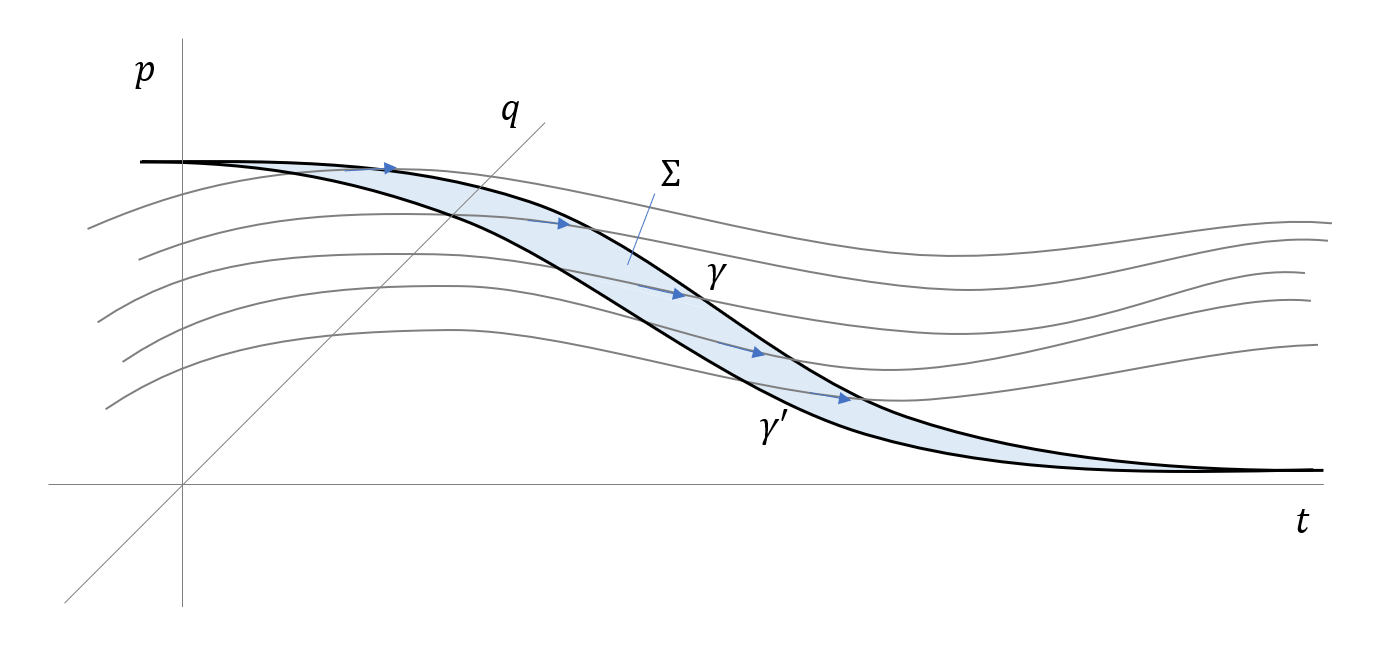
\includegraphics[width = 0.45\textwidth]{ActionNonOptimized.png} \\
	b 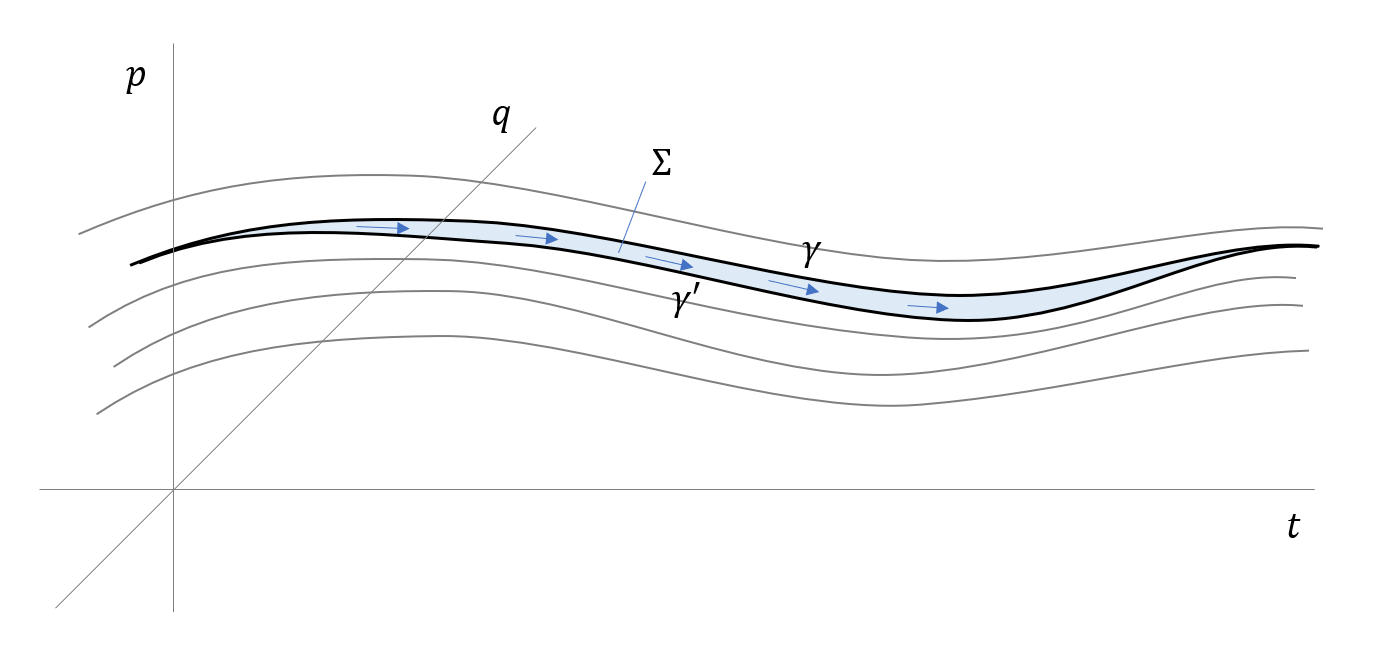
\includegraphics[width = 0.45\textwidth]{ActionOptimized.png}
	\caption{\footnotesize{The variation of the action is the flow of the displacement field $\vec{S}$ through the surface $\Sigma$ that sits between the path $\gamma$ and its variation $\gamma'$. In the second picture we see that the flow is zero if the path is an actual evolution of the system, since the displacement field will be parallel to the path $\gamma$ and therefore the surface $\Sigma$.}}\label{action}
\end{figure}

Now let us consider the variation of the line integral $\delta \int_{\gamma} \vec{\theta} \cdot d\vec{\gamma}$ caused by an infinitesimal change in the path. The original path $\gamma$ together with its variation $\gamma'$ form a contour $\partial \Sigma$ which encloses the surface $\Sigma$. We can therefore use Stokes' theorem to transform the line integral of $\vec{\theta}$ over $\partial \Sigma$ to a surface integral of the curl $\nabla \times \vec{\theta}$ over $\Sigma$. That is:
\begin{align*}
	\delta \int_{\gamma} \vec{\theta} \cdot d\vec{\gamma} 
	&= \int_{\gamma} \vec{\theta} \cdot d\vec{\gamma} - \int_{\gamma'} \vec{\theta} \cdot d\vec{\gamma'} \\
	&= \oint_{\partial \Sigma} \vec{\theta}  \cdot d\vec{\gamma} \\
	&= \iint_{\Sigma} \left( \nabla \times \vec{\theta} \right) \cdot d\vec{\Sigma} \\
	&= - \iint_{\Sigma} \vec{S} \cdot d\vec{\Sigma}.
\end{align*}
Note that, precisely because $\vec{S}$ is divergence-free, it doesn't matter which particular surface $\Sigma$ we pick, as long as its contour $\partial \Sigma$ consists of $\gamma$ and $\gamma'$.

The variation of the action, then, corresponds to the flow of $\vec{S}$ through $\Sigma$. It tells us how many actual evolutions go through the surface. Note that if $\gamma$ is an evolution of the system, it is always tangent to $\vec{S}$. This means that the surface $\Sigma$ enclosed by $\gamma$ and its infinitesimal variation is also tangent to $\vec{S}$ and therefore $\vec{S} \cdot d\vec{\Sigma} = 0$. Which means the actual evolutions are those paths $\gamma$ for which
\begin{equation}
	\delta \int_{\gamma} \vec{\theta} \cdot d\vec{\gamma} = 0.
\end{equation}
This recovers the principle of stationary action.

The action principle, then, is a direct consequence of the divergence-free nature of the displacement field $\vec{S}$. Every evolution $\gamma$ is a field line of $\vec{S}$. Any infinitesimal surface $\Sigma$ enclosed by an evolution and its variation, then, will also be tangent to the displacement field $\vec{S}$ and therefore the surface integral of $\vec{S}$ through $\Sigma$ will be zero. Given that $\vec{S}$ is divergence-free, the integral through $\Sigma$ can be expressed as the line integral of the vector potential $\vec{\theta}$ over the contour of $\Sigma$. Asking for a stationary action means asking for the flow of $\vec{S}$ to be zero across the surface given by the path and its variation, which happens only if the path is tangent to $\vec{S}$ and is therefore an evolution. In practice, the principle of stationary action is a very roundabout way to ask that the path be always tangent to the displacement vector field.

\subsection{Discussion}

Before proceeding to the more general case, there are two important things to note.

First of all, the true (and only) physical content of the discussion lies in condition \ref{Detrev_assumptions} that assumes deterministic and reversible motion. The displacement field $\vec{S}$ and its properties are the only mathematical entities that are directly physically meaningful. The vector potential $\vec{\theta}$ is not uniquely defined by condition \ref{Detrev_assumptions}, though it is extremely useful as it allows us to map the space of all possible displacement fields of interest with a single ``scalar'' function $H$, the time component of the vector potential.

Since the Lagrangian is equal to the scalar product between the displacement along a path $\frac{d\vec{\gamma}}{dt}$ and the vector potential $\vec{\theta}$, it suffers all the problems of the vector potential: it is not unique and its value is not directly physically meaningful. The same is true for the action itself. While the Lagrangian and the action are clearly useful tools in physics, this result warrants caution in relying exclusively on them to understand the physical relevance and meaning of a theory.

The second point is that our geometrical and physical interpretation works for all Hamiltonians. Technically, not all Hamiltonian systems admit a Lagrangian, as one needs an invertible map between conjugate momentum $p$ and the velocity $\frac{dq}{dt}$. For example, the following Hamiltonian
\begin{equation}
	H = c |p^i|
\end{equation}
is the one for a free photon treated as a particle. This gives us
\begin{equation}
	\frac{dq}{dt}= c \frac{p}{|p|}
\end{equation}
which means the velocity allows us to recover the direction of the conjugate momentum, but not its norm (i.e. the trajectory of a photon is not enough to recover its full state). In these cases, the Lagrangian approach cannot be applied because $\vec{\theta} \cdot \frac{d\vec{\gamma}}{dt}$ cannot be expressed as a function of position and velocity. Yet, if we express $L(q,p,t)$ in terms of conjugate momentum instead of velocity, the modified version of the variational principle still works.

Note that the failure can happen in the reverse direction too: there are Lagrangian systems for which we cannot express the Hamiltonian in terms of conjugate momentum. However, these are exactly the cases where the action principle fails to yield a single solution. Therefore we have the following points:
\begin{enumerate}
	\item the only Lagrangian systems in which the action principle yields a single solution are the ones that admit a Hamiltonian formulation;
	\item all Hamiltonian systems admit an action principle formulation, even if they do not admit a Lagrangian.
\end{enumerate}

In our view, this is enough evidence to conclude that the Hamiltonian setting in the extended phase space is the most natural to understand the action principle.

\section{Multiple degrees of freedom}

All our previous points will hold true in the generalization to multiple degrees of freedom. The only additional key insight is that determinism and reversibility will apply to each independent degree of freedom, meaning that we do not only preserve the total number of states of the system, but also that the total number of states is the product of the configurations given by each independent degree of freedom.

To express this requirement, the tools provided by differential calculus are not enough. We need elements of differential geometry, particularly symplectic geometry and contact manifolds. To make the treatment more appropriate for a physics audience, we are going to use a notation that parallels Einstein notation for general relativity. \footnote{The main differences are as follows. The vector basis will be noted as $e_a$ instead of $\frac{\partial}{\partial x^a}$. The covector basis will be noted as $e^a$ instead of $dx^a$. The exterior derivative will be noted as $\partial$ (e.g. $\partial \omega$) instead of $d$ (e.g. $d \omega$).}

\subsection{Hamiltonian reformulation}

Our system will be now composed of $N$ independent degrees of freedom. This means that we can chart all states at all times using $2N + 1$ variables $\xi^a = \{ q^i, p_i, t\}$. We will use $\xi^a$ when we want to span all variables; $q^i$ and $p_i$ when we want to span the position or the momentum of all degrees of freedom.

As before, we will have a displacement field
\begin{equation}
	\vec{S} = \frac{d\xi^a}{dt} e_{a} = \frac{dq^i}{dt} e_{q^i} + \frac{dp_i}{dt} e_{p_i} + \frac{dt}{dt} e_t.
\end{equation}
However, unlike in the single degree of freedom case, $\vec{S}$ is not the object used fully characterize the geometry of the space.

The main idea is that we want to be able to quantify the number of states identified by each degree of freedom. As degrees of freedom are bi-dimensional, this means quantifying the areas of two-dimensional surfaces. Therefore we introduce the rank-2 tensor
\begin{equation}
	\omega = \omega_{ab} \, e^a \otimes e^b,
\end{equation}
which we call the state counting tensor. The idea is that a pair of vectors $\vec{v}$ and $\vec{w}$ will identify a parallelogram in phase space and 
\begin{equation}
	\omega(\vec{v}, \vec{w}) = \omega_{ab} v^a w^b
\end{equation}
quantifies the number of states over its surface.

The tensor $\omega$ will need to satisfy additional conditions to be physically meaningful. First of all, it will need to be anti-symmetric. The parallelogram identified by $\vec{v}$ and $\vec{w}$ in that order will be the same as the one identified by $\vec{w}$ and $\vec{v}$ therefore the area is the same. However, the switch changes handedness, and therefore will introduce a minus sign. Therefore we have:
\begin{equation}
	\omega(\vec{v}, \vec{w}) = - \omega(\vec{w}, \vec{v}).
\end{equation}
Since the rank-2 tensor is anti-symmetric, it can be understood as a two-form in differential geometry. Only the components below the diagonal are independent, which means $\sum_1^{2N}i =N(2N+1)$ independent components.

The form $\omega$ will also be closed, meaning
\begin{equation}\label{mdof_closed_form}
	\oiint \omega = 0
\end{equation}
over all closed surfaces. In fact, consider a parallelepiped. Given that the degrees of freedom are independent, and we have deterministic and reversible motion, two opposite sides will contain the same number of states. Given that the two opposite sides will have opposite orientation, their total contribution will be zero. This logic can be extended to all three-dimensional differential volumes, as they can be decomposed into infinitesimal parallelepiped.

Since $\omega$ is closed, in every contractible region it can be expressed as the exterior derivative of a covector $\theta$. We have
\begin{equation}
\begin{aligned}
	\theta &= \theta_a e^a = \theta_{q^i} e^{q^i} + \theta_{p_i} e^{p_i} + \theta_t e^t \\
	\omega &= - \partial \theta = - \left( \partial_a \theta_b - \partial_b \theta_a \right) e^a \otimes e^b
\end{aligned}
\end{equation}
The minus sign is the convention in symplectic geometry.

In the generalization we need to distinguish between vectors, like $\vec{S}$, covectors, like $\theta$, and two-forms, like $\omega$. The single degree of freedom used only three variables, therefore to each parallelogram in $\{q, p, t\}$ there is only one perpendicular direction, which allows us to blur the line between the objects in the following way:
\begin{itemize}
	\item for each covector $\theta$ we can find a vector $\vec{\theta}$ such that $\theta(\vec{S})=\vec{\theta} \cdot \vec{S}$;
	\item for each two-form $\omega$ we can find a vector $\vec{\omega}$ such that $\omega(\vec{v}, \vec{w}) = \vec{\omega} \cdot \vec{v} \times \vec{w}$.
\end{itemize}
This is what allows us to think only in terms of vectors. This cannot be done in the general case. In particular, the generalization of the curl is no longer an operation between vectors, but an operation that takes a one-form and returns a two-form.

Now we need to further characterize $\omega$. Each pair of variables $q^i$, $p_i$ forms an independent degree of freedom. This means that only surfaces spanned by matching position and momentum will define actual states, while all other combinations will not define any state. Therefore:
\begin{equation}\label{canonical_conditions}
\begin{aligned}
	\omega(e^{q^i}, e^{p_j}) = \omega_{q^i p_j} &= \delta^i_j = - \omega_{p_j q^i} \\
	\omega(e^{q^i}, e^{q^j}) = \omega_{q^i q^j} &= 0 \\
	\omega(e^{p_i}, e^{p_j}) = \omega_{p_i p_j} &= 0
\end{aligned}
\end{equation}
Of the $N(2N+1)$ independent components given the anti-symmetry requirement, the first condition sets $N^2$ of these while the last two set $N(N-1)/2$ independent components each. This totals $N(2N-1) = \sum_1^{2N-1}i$ independent components.

Assuming determinism and reversibility, time evolution contributes no new states, it just moves them in time. That is, no states appear or disappear from any degree of freedom. The displacement field doesn't define any state, no matter which other vector it is paired with. Mathematically, we say that the displacement kills the form
\begin{align}\label{mdof_displacement_kills}
	\omega(\vec{S}, \cdot) = 0.
\end{align}
This sets another $2N$ components (since $\omega(\vec{S}, \vec{S}) = 0$ is already set by anti-symmetry). All independent components are now set.

Those familiar with symplectic and contact geometry will recognize that conditions \ref{canonical_conditions} mean that $q^i$ and $p_i$ are canonical coordinates and, by Darboux's theorem, we will be able to write the covector potential as
\begin{equation}\label{mdof_potential_expression}
	\theta = p_i e^{q^i} - H e^t.
\end{equation}
Let us convince ourselves of this result by constructing a proof that is similar to what we have done for the single degree of freedom.

First, we express \ref{canonical_conditions} in terms of the covector potential. We have:
\begin{equation}\label{canonical_potential_conditions}
\begin{aligned}
	\omega(e^{q^i}, e^{p_j}) &= (-\partial\theta)_{q^i p_j} = -(\partial_{q^i}\theta_{p_j} - \partial_{p_j}\theta_{q^i}) = \delta^i_j \\
	\omega(e^{q^i}, e^{q^j}) &= (-\partial\theta)_{q^i q^j} = -(\partial_{q^i}\theta_{q^j} - \partial_{q^j}\theta_{q^i}) = 0 \\
	\omega(e^{p_i}, e^{p_j}) &= (-\partial\theta)_{p_i p_j} = -(\partial_{p_i}\theta_{p_j} - \partial_{p_j}\theta_{p_i}) = 0
\end{aligned}
\end{equation}
We can use our gauge freedom to set $\theta_{p_1} = 0$, much in the same way we did for the simpler case. We now have $\partial_{q^1} \theta_{p_1} = 0$ and, by the first condition, $\partial_{p_1} \theta_{q^1} = 1$. Integrating, we have $\theta_{q^1} = p_1 + g(q^i, p_2, p_3, ..., t)$ where $g$ is an arbitrary function which we can set to zero. Like in the single degree of freedom, we can do this because $g$ does not depend on $p_1$, so it can be eliminated with a gauge transformation that does not change $\theta_{p_1}$. Therefore we have:
\begin{equation}
	\theta = p_1 e^{q^1} + 0 e^{p_1} + \theta_{q^2} e^{q^2} + \theta_{p_2} e^{p_2} + ... + \theta_{t} e^{t}.
\end{equation}

Note that the components for the first degree of freedom do not depend on the other degrees of freedom. That is, for all $i>1$, $\partial_{q^i} \theta_{q^1} = \partial_{p_i} \theta_{q^1} = \partial_{q^i} \theta_{p_1} = \partial_{p_i} \theta_{p_1} = 0$. But by using conditions \ref{canonical_potential_conditions}, we find that the converse is true as well: the components of all other degrees of freedom do not depend on the first. That is, for all $i>1$, $\partial_{q^1} \theta_{q^i} = \partial_{p_1} \theta_{q^i} = \partial_{q^1} \theta_{p_i} = \partial_{p_1} \theta_{p_i} = 0$.

We can then use, again, our gauge freedom with a function that does not depend on the first two variables to set $\theta_{p_2} = 0$. And, with the same reasoning, we will be able to set $\theta_{q^2} = p_2$. And then, again, find that the first two degrees of freedom do not depend on the others, etc. At the end, we will find \ref{mdof_potential_expression}.

At this point, we calculate $\partial\theta(S, \cdot ) $. The components of $\partial\theta$ are:
\begin{equation*}
	(\partial\theta)_{ab} = \begin{bmatrix}
		0 & \delta^j_i & - \partial_{q^i} H \\
		-\delta^i_j & 0 & - \partial_{p_i} H \\
		\partial_{q^j} H & \partial_{p_j} H & 0
	\end{bmatrix}
\end{equation*}
We have
\begin{align*}
	\partial\theta(S, \cdot )  &= S^a (\partial\theta)_{ab} e^b = 0 \\
	&= (S^{q^i}(\partial\theta)_{q^ib} + S^{p_i}(\partial\theta)_{p_ib} + S^{t}(\partial\theta)_{tb}) e^b \\
	&= (S^{q^i}(\partial\theta)_{q^iq^j} + S^{p_i}(\partial\theta)_{p_iq^j} + S^{t}(\partial\theta)_{tq^j}) e^{q^j} + \\
	& (S^{q^i}(\partial\theta)_{q^ip_j} +  S^{p_i}(\partial\theta)_{p_ip_j} + S^{t}(\partial\theta)_{tp_j}) e^{p_j} + \\
	& (S^{q^i}(\partial\theta)_{q^it} + S^{p_i}(\partial\theta)_{p_it} + S^{t}(\partial\theta)_{tt}) e^t \\
	&= (-S^{p_i}\delta^i_j + S^{t}\partial_{q^j} H ) e^{q^j} + \\
	& (S^{q^i}\delta^j_i +  S^{t}\partial_{p_j} H) e^{p_j} + \\
	& (-S^{q^i} \partial_{q^i} H - S^{p_i} \partial_{p_i} H) e^t \\
\end{align*}

All components must be zero, therefore we have the following three equations:
\begin{align*}
	S^{p_j} &= S^{t} \partial_{q^j} H \\
	S^{q^j} &= - S^{t}\partial_{p_j} H \\
	-S^{q^i} \partial_{q^i} H - S^{p_i} \partial_{p_i} H &= S^{t}\partial_{p_i} H \partial_{q^i} H - S^{t} \partial_{q^i} H \partial_{p_i} H = 0
\end{align*}
Note that the last expression is not a new equation: it is identical to zero given the previous two equations. Since $S^t = 1$, we have:
\begin{align*}
	S^{p_j} &= \partial_{q^j} H \\
	S^{q^j} &= - \partial_{p_j} H
\end{align*}
which recovers Hamilton's equations for multiple degrees of freedom.

Once again, we have found that the whole physical content is included in condition \ref{Detrev_assumptions}. The geometry in the extended phase space is fully specified by the state counting form $\omega$. This does not define lengths and angles, like the metric tensor does for a more standard geometric setting. It defines areas of two-dimensional surfaces in terms of states, and angles between two-dimensional surfaces in terms of the degree of independence between degrees of freedom. What the equations say is simply that states move in time at the same rate (i.e. $\frac{dt}{dt} = 1$) with a deterministic and reversible flow (i.e. no states are created or destroyed on any independent degree of freedom).

\subsection{Action principle}
Having reformulated Hamiltonian mechanics in the extended phase space using the language of differential geometry, the geometrical interpretation of the action principle is essentially the same.

The Lagrangian is equal to the potential covector applied to the displacement along a generic path. That is
\begin{equation}
\begin{aligned}
L &= \theta\left(\frac{d\vec{\gamma}}{dt}\right) = \theta_a \frac{d\xi^a}{dt} \\
&= p_i \frac{dq^i}{dt} + 0 \frac{dp_i}{dt} - H \frac{dt}{dt} \\
&= p_i \frac{dq^i}{dt} - H.
\end{aligned}
\end{equation}

As before, we will consider the variation of the line integral $\delta \int_{\gamma} \theta(d\vec{\gamma})$, which can be expressed as
\begin{equation}
	\begin{aligned}
		\int_A^B \theta(d\vec{\gamma}) &= \int^{t_1}_{t_0} \theta\left(\frac{d\vec{\gamma}}{dt}\right) dt \\
		&= \int^{t_1}_{t_0} \left(p_i \frac{dq^i}{dt} - H \right) dt
	\end{aligned}
\end{equation}
The original path $\gamma$ together with its variation $\gamma'$ form a contour $\partial \Sigma$. We can then use Stokes' theorem to transform the line integral of $\theta$ to a surface integral of its exterior derivative. That is:
\begin{align*}
	\delta \int_{\gamma} \theta(d\vec{\gamma}) = 
	&= \int_{\gamma} \theta(d\vec{\gamma}) - \int_{\gamma'} \theta(d\vec{\gamma}') \\
	&= \oint_{\partial \Sigma} \theta(d\vec{\gamma}) \\
	&= \iint_{\Sigma} \partial \theta (d\Sigma) \\
	&= - \iint_{\Sigma} \omega(d\Sigma).
\end{align*}
At each point, one side of $d\Sigma$ will be $d\vec{\gamma}$, therefore $\omega(d\Sigma) = \omega(d\vec{\gamma}, d\vec{\lambda})$ where $d\vec{\lambda}$ is the direction of the variation. If $\gamma$ is an actual evolution, $d\vec{\gamma} = \vec{S} dt$ and, by \ref{mdof_displacement_kills}, we have
\begin{equation}
	\begin{aligned}
	\delta \int_{\gamma} \theta (d\vec{\gamma}) &= - \iint_{\Sigma} \omega(d\Sigma) \\
	&= - \iint_{\Sigma} \omega(d\vec{\gamma}, d\vec{\lambda}) \\
	&= - \iint_{\Sigma} \omega(\vec{S}, d\vec{\lambda}) dt \\
	&= - \iint_{\Sigma} 0 = 0
	\end{aligned}
\end{equation}

The action principle, then, is a direct consequence of the geometry set by \ref{mdof_closed_form} and \ref{mdof_displacement_kills}, which is the generalization of the divergence-free nature of the displacement field $\vec{S}$. Every evolution $\gamma$ is a field line of $\vec{S}$. Any infinitesimal surface $d\Sigma$ enclosed by an evolution and its variation, then, will also be tangent to the displacement field $\vec{S}$ and therefore will contribute no states, $\omega(d\Sigma)$ will be zero. Given that $\omega$ is closed, the integral over $\Sigma$ can be expressed as the line integral of the covector potential $\theta$ over the contour of $\Sigma$.

\subsection{Discussion}

Apart from the technicalities needed to properly frame the problem, multiple degrees of freedom do not add much conceptually. All geometrical and physical content within the theory is about counting states and keeping track of how they move in time, which is done by the two-form $\omega$. As before, the assumption of deterministic and reversible evolution does all the work.

The additional key assumption is that the degrees of freedom must be independent. If the degrees of freedom were not independent, then the number of states within a four-dimensional parallelepiped would not be given by the product of the count of states on the sides. We would need additional structure. If the degrees of freedom started independent but didn't remain so, the displacement field $\vec{S}$ would only preserve the count of states of volumes, not over each degree of freedom, and therefore $\omega(\vec{S}, \cdot) \neq 0$.

The comments on the lack of strict physicality for the values of the Lagrangian and the action remain unchanged. They both depend on a choice of gauge. The comment on the centrality of the extended phase space to understand the action principle is only reinforced. Additionally, note that by changing $t$ to $ct$ expression \ref{mdof_potential_expression} becomes
\begin{equation}\label{mdof_potential_relativistic}
	\theta = p_i e^{q^i} - \frac{H}{c} e^{ct}.
\end{equation}
which bears striking resemblance to the relativistic four-momentum. While it goes outside the scope of this article, the idea is that, in this setting, we already have some pre-relativistic features, even though we have not introduced a metric tensor.

\section{Conclusion}

We have given a geometrical interpretation of the principle of stationary action that is also fully physically motivated by the assumption of deterministic and reversible evolution. The key insight is that a path $\gamma$ and a variation form a closed curve which encloses a surface $\Sigma$. If the path is an actual evolution for the system, all states flow along the surface $\Sigma$, not through it. Using Stokes' theorem, the zero flow condition through the surface $\Sigma$ is transformed to a zero integral condition on its boundary (i.e. on the path $\gamma$ and its variation) leading to the principle of least action.

We have seen that both the Lagrangian and the action depend on the potential, which means they are gauge dependent. This makes the numerical values of those objects not strictly physical. We have seen that the interpretation given also works for those Hamiltonian systems that do not have a corresponding Lagrangian, meaning that the most general expression for the action principle lies on the extended-phase-space Hamiltonian formulation of classical mechanics. We have seen that elements from symplectic and contact geometry are needed for the generalization to multiple degrees of freedom and that they can be formulated in a language that is less abstract and closer to physics conventions.

All considered, we believe this way of looking at classical mechanics provides a more complete characterization and better insights than the usual treatments.

\bibliography{bibliography}


\end{document}